\algblockdefx{RepeatUntil}{EndRepeatUntil}{\textbf{repeat until}}{}
\algnotext{EndRepeatUntil}

\section{Semi-Analytic Primal Solver}
\label{sec:sap_solver}

Inspired by Newton's method, our Semi-Analytic Primal Solver (SAP) seeks to monotonically decrease the primal cost $\ell_p(\mf{v})$ at each iteration, as outlined in Algorithm \ref{alg:sap}
\begin{algorithm}[H]
	\caption{The Semi-Analytic Primal Solver (SAP)}	
	  \label{alg:sap}
	  \begin{algorithmic}[1]
		  \State Initialize $\mf{v}_m \gets \mf{v}_0$
		  \RepeatUntil $~\Vert\tilde{\nabla}\ell_p\Vert < \varepsilon_a + \varepsilon_r\max(\Vert\tilde{\mf{p}}\Vert,\Vert\tilde{\mf{j}_c}\Vert)$, Eq. \eqref{eq:stopping_criteria}
			  \State $\Delta\mf{v}_{m} = -\mf{H}^{-1}(\mf{v}_m)\nabla_\mf{v}\ell_p(\mf{v}_m)$ \label{op:Newton_iteration}
			  \State $\displaystyle \alpha_m = \argmin_{t\in\mathbb{R}^{++}} \ell_p(\mf{v}_m + t \Delta\mf{v}_{m})$
			  \State $\displaystyle \mf{v}_{m+1} = \vf{v}_m + \alpha_{m}\Delta\mf{v}_{m}$
		  \EndRepeatUntil
		  \State\Return $\{\mf{v}$, $\bgamma=P_\mathcal{F}(\vf{y}(\mf{v}))\}$
	  \end{algorithmic}
\end{algorithm}

The SAP iterations require $\mf{H}(\mf v)\succ 0$ at all iterations.  At points
of differentiability, $\mf{H}(\mf v)$ is simply set equal to the Hessian of the
cost function. In general, $\mf{H}(\mf v)$ is evaluated using a partition of its
domain. For each set in the partition, the gradient is differentiable on the
interior, and the Hessian admits a simple formula. Outside the interior, we
evaluate $\mf{H}(\mf v)$ by using the Hessian formula derived for the interior.
This procedure provides a globally valid definition for $\mf{H}(\mf v)$. The
partition is described in Appendix
\ref{app:analytical_inverse_dynamics_derivations}. The Hessian formula are given
in Appendix \ref{app:gradients_derivation}. Our convergence analysis in Appendix
\ref{app:sap_converge} also accounts for this definition.

As shown in Appendix \ref{app:sap_converge}, SAP globally convergences at least
at a linear-rate. Further, SAP exhibits quadratic convergence when $\nabla^2
\ell_p$ exists in a neighborhood of the optimal $\mf{v}$. In practice, we
initialize SAP with the previous time-step velocity $\mf{v}_0$. The stopping
criteria is discussed below in Section \ref{sec:stopping_criteria}.

\subsection{Gradients}
\label{sec:gradients}

We provide a detailed derivation of the gradients in Appendix
\ref{app:gradients_derivation}. Here we summarize the main results required for
implementation. The gradient of the primal cost $\ell_p$ reduces to the balance
of momentum
\begin{equation*}
	\nabla_\mf{v}\ell_p(\mf{v}) = \mf{A}(\mf{v}-\mf{v}^*) - \mf{J}^T\bgamma(\mf{v}),
\end{equation*}
where $\bgamma(\mf{v})=P_\mathcal{F}(\vf{y}(\mf{v}))$ is given by the analytical
inverse dynamics \eqref{eq:analytical_y_projection}. We define matrix
$\mf{G}\succeq 0$ that evaluates to $-\nabla_{\mf{v}_c}\bgamma$ where
$P_\mathcal{F}(\mf{y}(\mf{v}))$ is differentiable. Otherwise $\mf{G}$ extends
our analytical expressions as outlined in Appendix
\ref{app:gradients_derivation}. Matrix $\mf{G}$ is a block diagonal matrix where
each the diagonal block for the $i\text{-th}$ contact is a $3\times 3$ matrix.

In total, we evaluate $\mf{H}$ via
\begin{equation}
	\mf{H} = \mf{A} + \mf{J}^T\mf{G}\,\mf{J},
\end{equation}
which is strictly positive definite since $\mf{A}\succ 0$.

\subsection{Line Search}

The line search algorithm is critical to the success of SAP given that $\nabla
\ell_p(\mf{v})$ can rapidly change during contact-mode transitions.  We explore
two line search algorithms: an approximate backtracking line search with
Armijo's stopping criteria and an exact (to machine epsilon) line search.

At the $m\text{-th}$ Newton iteration, backtracking line search starts with a
maximum step length of $\alpha_\text{Max}$ and progressively decreases it
by a factor $\rho \in (0, 1)$ as $\alpha\gets\rho\alpha$ until Armijo's
criteria \cite[\S 3.1]{bib:nocedal2006numerical} is satisfied. We write Armijo's
criteria as $~\ell_p(\mf{v}^m + \alpha \Delta\mf{v}^{m}) < \ell_p(\mf{v}^m) +
c\,\alpha\,d\ell_p/d\alpha(\mf{v}^m)$. Typical parameters we use are
$\rho=0.8$, $c=10^{-4}$ and $\alpha_\text{Max}=1.5$.

For the exact line search we use the method \verb;rtsafe; \cite[\S
9.4]{bib:numerical_recipes} to find the unique root of $d\ell/d\alpha$. \verb;rtsafe; is a one-dimensional
root finder that uses the Newton-Raphson method and switches to bisection
when an iterate falls outside a search bracket or
when convergence is slow. The fast computation of derivatives we show next
allows us to iterate $\alpha$ to machine precision at a negligible impact on the
computational cost. In practice, this is our preferred algorithm since it allows
us to use very low regularization parameters without having to tune tolerances
in the line search. Moreover, we observe 15\%-35\% performance improvement when
compared to the backtracking line search.

\subsection{Efficient Analytical Derivatives For Line Search}

The algorithm \verb;rtsafe; requires the first and second directional
derivatives of $\ell_p$, while the
backtracking method only requires the first derivative to verify Armijo's
stopping criteria. We show how to compute these derivatives efficiently in
$\mathcal{O}(n)$ operations. Defining $\ell(\alpha) =
\ell_p(\mf{v}+\alpha\Delta\mf{v})$, we compute first and second derivatives as
\begin{align*}
	\frac{d\ell}{d\alpha}&=\Delta\mf{v}^T\nabla_\mf{v}\ell(\alpha),\\
	\frac{d^2\ell}{d\alpha^2}&=\Delta\mf{v}^T\mf{H}(\alpha)\Delta\mf{v}.
\end{align*}

Using the gradients from Section \ref{sec:gradients}, we can write
\begin{align*}
	\frac{d\ell}{d\alpha}(\alpha)=\Delta\mf{v}^T\mf{A}(\mf{v}(\alpha)-\mf{v}^*)-\Delta\mf{v}^T\mf{J}^T\bgamma.
\end{align*}
These are computed efficiently by first calculating the change in velocity
$\Delta\mf{v}_c:=\mf{J}\Delta\mf{v}$ and change of momentum $\Delta\mf{p} :=
\mf{A}\Delta\mf{v}$. The calculation is then completed via 
\begin{align*}
	\frac{d\ell}{d\alpha}(\alpha)=\Delta\mf{p}^T(\mf{v}(\alpha)-\mf{v}^*)
	-\Delta\mf{v}_c^T\bgamma(\alpha),
\end{align*}
which only requires dot products that can be computed in $\mathcal{O}(n_v)$ and
$\mathcal{O}(n_c)$ respectively. Similarly for the second derivatives
\begin{align*}
	\frac{d^2\ell}{d\alpha^2}(\alpha)=\Delta\mf{v}^T\Delta\mf{p} + \Delta\mf{v}_c^T
	\mf{G}\Delta\mf{v}_c.
\end{align*}

Notice the first term on the right can be precomputed before the line search
 starts, while the second term only involves $\mathcal{O}(n_c)$ operations given
 the block diagonal structure of $\mf{G}$.

\subsection{Problem Sparsity}
\label{sec:problem_sparsity}

The matrix $\mf{H}(\mf{v}^m)$ inherits a block sparse structure from
the specific contact configuration of the problem. 
We exploit this structure using a supernodal Cholesky factorization \cite[\S
9]{bib:davis2016survey}. Implementing this factorization requires construction
of a \emph{junction tree}.  For this we apply the algorithm in
\cite{bib:smail2017junction}, using cliques of $\mf{H}$ as input. We
use the implementation from the Conex solver \cite{bib:permenter2020}.

The block sparsity of $\mf{H}$  is best described with an example. We organize
our multibody systems as a collection of articulated \emph{tree structures}, or
a \emph{forest}. Consider the system in Fig. \ref{fig:sparsity_example}.
\begin{figure}[!h]
	\centering
	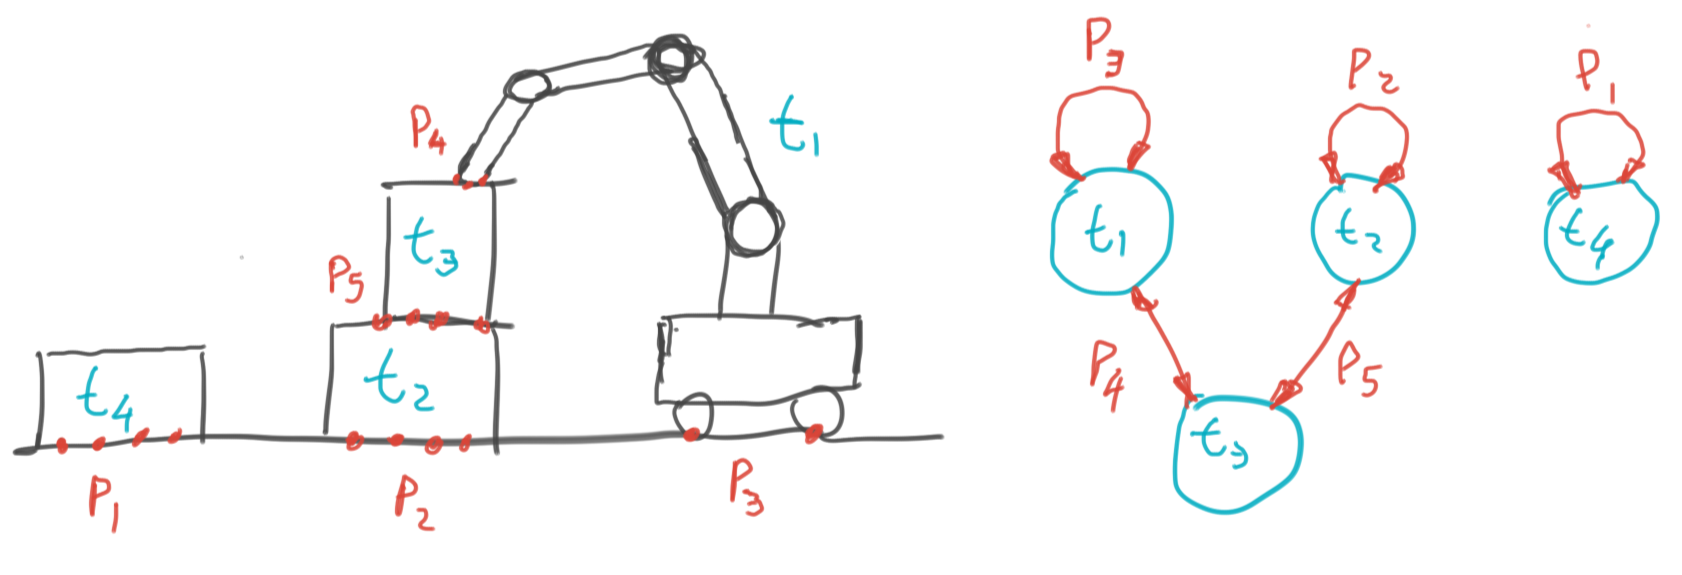
\includegraphics[width=0.7\columnwidth]{figures/sparsity_example.png}
	\caption{\label{fig:sparsity_example} 
	An example of a sparsity pattern commonly encountered in the
	simulation of robotic mechanical systems. The graph on the right puts
	\textit{trees} as nodes and contact \textit{patches} as edges.}
\end{figure}
In this example, a robot arm mounted on a mobile base constitutes its own tree,
here labeled $t_1$. The number of degrees of freedom of the $t\text{-th}$ tree
will be denoted with $n_t$. A free body is the common case of a tree with
$n_t=6$. In general, matrix $\mf{A}$ has a
block diagonal structure where each diagonal block corresponds to a tree.

We define as \textit{patches} a collection of contact pairs between two
trees. Each contact pair corresponds to a single cone constraint in our
formulation. The set of constraint indexes that belong to patch $p$ is
denoted with $\mathcal{I}_p$ of size (cardinality) $|\mathcal{I}_p| = r_p$.
Figure~\ref{fig:sparsity_example} shows the corresponding graph where nodes
correspond to trees and edges correspond to patches.

Generally, the Jacobian is sparse since the relative contact velocity only
involves velocities of two trees in contact. When rows are condensed by patches
and columns by trees, the Jacobian exhibits a sparse block structure. For the
example in Fig.~\ref{fig:sparsity_example}, the Jacobian looks
like\\\\
\begin{equation}
	\mf{J}=\quad
	\begin{bmatrix}
		\tikzmark{J_topleft}\mf{0} & 
		\mf{0} & \mf{0} & \mf{J}_{\rr{1}\cc{4}}\tikzmark{J_topright}\\		
		\mf{0} & \mf{J}_{\rr{2}\cc{2}} & \mf{0} & \mf{0}\\
		\mf{J}_{\rr{3}\cc{1}} & \mf{0} & \mf{0} & \mf{0}\\
		\mf{J}_{\rr{4}\cc{1}} & \mf{0} & \mf{J}_{\rr{4}\cc{3}} & \mf{0}\\
		\tikzmark{J_bottomleft}
		\mf{0} & \mf{J}_{\rr{5}\cc{2}} & \mf{J}_{\rr{5}\cc{3}} & \mf{0}		
	\end{bmatrix}
% Draw lil arrows on top and to the left.
\tikz[overlay,remember picture] {
	\draw[->,thick,color=cyan]
  ([yshift=3ex]J_topleft) -- ([yshift=3ex]J_topright) node[midway,above]
  {\scriptsize $t$}; 
  \draw[->,thick,color=red]
  ([yshift=1.5ex,xshift=-3ex]J_topleft) -- ([xshift=-3ex]J_bottomleft)
  node[near end,left] {\scriptsize $p$};}	
\end{equation}
\RedHighlight{Consider making this part of Fig. \ref{fig:sparsity_example}}\\
where each non-zero block is the Jacobian $\mf{J}_{\rr{p}\cc{t}}$ of size
$3r_p\times n_t$.

Finally, since $\mf{A}$ is block diagonal, $\mf{H}$ inherits the sparsity
structure of $\mf{J}^T\mf{G}\mf{J}$. For our example, this is sketched in
\ref{fig:JTGJ_schematic}. Notice how the sparsity pattern of
$\mf{J}^T\mf{G}\mf{J}$ exactly matches the graph from Fig.
\ref{fig:sparsity_example}. Using this block structure, our supernodal Cholesky
factorization can take full advantage of specific optimizations for dense
algebra.
\begin{figure*}[!h]
	\centering
	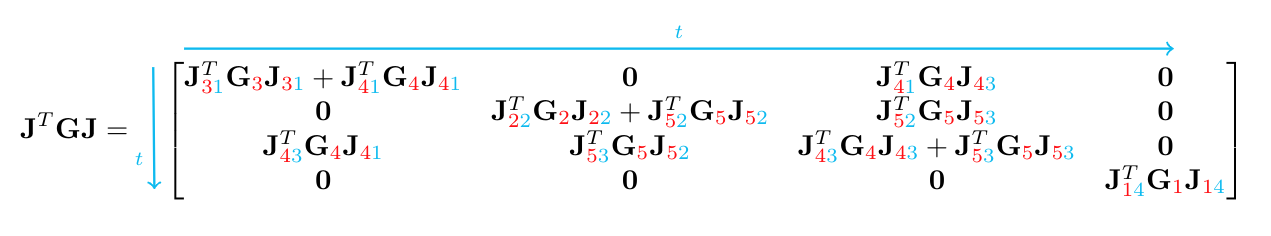
\includegraphics[width=0.8\textwidth]{figures/JTGJ_schematic.png}
	\caption{\label{fig:JTGJ_schematic} 
	Block sparsity of the $\mf{J}^T\mf{G}\mf{J}$ for the example illustrated in
	Fig. \ref{fig:sparsity_example}.}
\end{figure*}

\subsection{Stopping Criteria}
\label{sec:stopping_criteria}

To assess convergence, we monitor the norm of optimality condition for the
unconstrained problem (\ref{eq:primal_unconstrained})
\begin{equation*}
	\nabla\ell_p(\mf{v}) = \mf{A}(\mf{v}-\mf{v}^*) - \mf{J}^T\bgamma.
\end{equation*}

Notice that the components of $\nabla\ell_p$ have units of generalized momentum
$\mf{p}=\mf{M}\mf{v}$. Depending on the choice of generalized coordinates, the
generalized momentum components may have different units. In order to weigh all
components equally, we define the diagonal matrix $\mf{D} =
\text{diag}(\mf{M})^{-1/2}$ and perform the following change of variables
\begin{align}
	\tilde{\nabla}\ell_p &= \mf{D}\nabla\ell_p, \nonumber\\
	\tilde{\mf{p}} &= \mf{D}\mf{p}, \nonumber \\
	\tilde{\mf{j}}_c &= \mf{D}\mf{j}_c,
	\label{eq:scaled_momentum_quantities}
\end{align}
where we defined the generalized contact impulse $\mf{j}_c=\mf{J}^T\bgamma$.
With this scaling, all the new \emph{tilde} variables have the same units,
square root of Joules. Using these definitions, we write our stopping criteria
as
\begin{equation}
	\Vert\tilde{\nabla}\ell_p\Vert < \varepsilon_a + \varepsilon_r\max(\Vert\tilde{\mf{p}}\Vert,\Vert\tilde{\mf{j}_c}\Vert).
	\label{eq:stopping_criteria}
\end{equation}
where $\varepsilon_r$ is a dimensionless relative tolerance that we usually set
in the range from $10^{-6}$ to $10^{-3}$. The absolute tolerance $\varepsilon_a$
is used to detect rare cases where the solution leads to no contact and no
motion, typically due to external forces. We always set this tolerance to a
small number, $\varepsilon_a=10^{-16}$.
